\documentclass[journal,draftclsnofoot]{IEEEtran} 
\usepackage{graphicx}            %include pictures
\usepackage{amsmath}             %math functions
\usepackage{siunitx}             %fills in si units and order of magnitudes (mm, micro)
\usepackage[hyphens]{url}        %websites, hyphenated when longer than a line
\usepackage{cleveref}
\usepackage{hyperref}
\usepackage{algorithm2e}
%%%%%%%%%%%%%%%%%%%%%%%%%%%%%%%%%%%%%%%%%%%%%%%%%%%%%%%%%%%%%%%%%%%%%%%%%%%%%%%%%%%%%%%%%%%%%%%%%%%%%%%%%%%%%%%%%%%%
\begin{document}
\title{ELEN 4020 Project - Comparison of Parallel Equi-Join using MPI and OpenMP}
\author{Uyanda~Mphunga~-~1168101,~Darren Blanckensee~-~1147279,~Ashraf Omar~-~710435 and~Amprayil~Joel~Oommen~-~843463
\thanks{School of Electrical \& Information Engineering, University of the
Witwatersrand, Private Bag 3, 2050, Johannesburg, South Africa}
}
\maketitle
\pagestyle{plain}
\begin{abstract}

\end{abstract}
%%%%%%%%%%%%%%%%%%%%%%%%%%%%%%%%%%%%%%%%%%%%%%%%%%%%%%%%%%%%%%%%%%%%%%%%%%%%%%%%%%%%%%%%%%%%%%%%%%%%%%%%%%%%%%%%%%%%%
\section{Introduction}
The join operation concerns the combining of two different tuples on a common join attribute \cite{Yu1998}. It is important in information systems, in particular the use of databases since the join operation is the most expensive operation in database query operations in terms of time and data-intensity \cite{Mishra1992}. This project explores two different approaches to performing a join of two very large tables. The problem is described in Section \ref{prob} and the two different approaches discussed in Sections \ref{mpi} and \ref{omp}. The method of experimentation is outlined in Section \ref{desc} and the results of the experiment are analysed in Section \ref{ana}. Section \ref{conc} reviews the project and concludes this document.
%%%%%%%%%%%%%%%%%%%%%%%%%%%%%%%%%%%%%%%%%%%%%%%%%%%%%%%%%%%%%%%%%%%%%%%%%%%%%%%%%%%%%%%%%%%%%%%%%%%%%%%%%%%%%%%%%%%%
\section{Problem Description}\label{prob}
The objective of this project is to perform an equi-join of two very large tables. An equi-join is a type of join that uses the equality operator as a basis for the join \cite{w3resource.com2018} that is if the join attribute in $R_{1}(A,B)$ is strictly equal to the join attribute in $R_{2}(A,C)$ the result of the join is inserted into a third table $R_{3}(A, B, C)$. An illustrated example can be seen in Figure \ref{fig:Equi-Join}.
\begin{figure}[htbp]
	\centering
		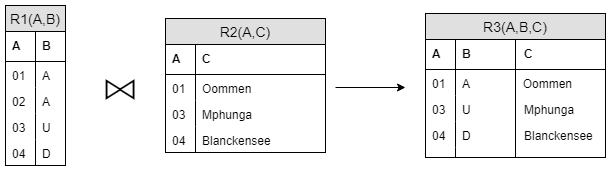
\includegraphics[width=0.4882\textwidth]{Equi-Join.png}
	\caption{An example of equi-join between two relational tables}
	\label{fig:Equi-Join}
\end{figure}
The join must be done using two different algorithms, one that is based in MPI (Message Passing Interface), and one that uses another high-level parallel programming model. The programming model chosen in this project is OpenMP. The two programmes need to be compared with one another in terms of speed-up and scalability when increasing the number of processors and nodes that the program uses. The MPI join algorithm being used is hash-join and the OpenMP join algorithm being used is merge-join. The speed-up comparison is performed by running the two programs with increasing number of processors and the scalability comparison is conducted by increasing the number of nodes the program uses in a cluster.

%%%%%%%%%%%%%%%%%%%%%%%%%%%%%%%%%%%%%%%%%%%%%%%%%%%%%%%%%%%%%%%%%%%%%%%%%%%%%%%%%%%%%%%%%%%%%%%%%%%%%%%%%%%%%%%%%%%%
\section{MPI Join Algorithm -- Hash-Join}\label{mpi}
An overview of the algorithm being used is listed in Algorithm \ref{algMPI}.
\begin{algorithm}
 \KwData{Table $R_{1}(A,B)$, Table $R_{2}(A,C)$}
 \KwResult{$R_{3}(A, B, C)$}
 \For{all key-value pairs in $R_{1}$}{
  read key\;
	calculate hash as sum(ASCII) of key\;
  calculate (hash\%(no. of processes - 1) + 1)\;
 }
send key-value pairs of $R_{1}(A,B)$ to slave nodes in vector\;
\For{all key-value pairs in $R_{2}$}{
  read key\;
	calculate hash as sum(ASCII) of key\;
  calculate (hash\%(no. of processes - 1) + 1)\;//This is to determine which slave node the key-value pair is sent to.
 }
send key-value pairs of $R_{2}(A,C)$ to slave nodes in vector\;
IN EACH SLAVE NODE:\\
\For{all key-value pairs in each vector}{
	\If{key from $R_{1}$ == key from $R_{2}$}{
		write key-value output to $R_{3}$
	}
}

 \caption{MPI Implementation of hash-join}
\label{algMPI}
\end{algorithm}
%%%%%%%%%%%%%%%%%%%%%%%%%%%%%%%%%%%%%%%%%%%%%%%%%%%%%%%%%%%%%%%%%%%%%%%%%%%%%%%%%%%%%%%%%%%%%%%%%%%%%%%%%%%%%%%%%%%%
\section{OpenMP Join Algorithm -- Merge-Join}\label{omp}
The OpenMP join algorithm being implemented is merge-join. The two table are sorted by join attribute. Then the table are scanned and join attributes are compared to one another. For an equi-join, if the join attribute of one entry is strictly equal to the join attribute of the other table's entry, the entries are joined in the output table \cite{Pavlo2017}.
%%%%%%%%%%%%%%%%%%%%%%%%%%%%%%%%%%%%%%%%%%%%%%%%%%%%%%%%%%%%%%%%%%%%%%%%%%%%%%%%%%%%%%%%%%%%%%%%%%%%%%%%%%%%%%%%%%%%
\section{Experiment Description}\label{desc}
%%%%%%%%%%%%%%%%%%%%%%%%%%%%%%%%%%%%%%%%%%%%%%%%%%%%%%%%%%%%%%%%%%%%%%%%%%%%%%%%%%%%%%%%%%%%%%%%%%%%%%%%%%%%%%%%%%%%
\section{Analysis of Results}\label{ana}
%%%%%%%%%%%%%%%%%%%%%%%%%%%%%%%%%%%%%%%%%%%%%%%%%%%%%%%%%%%%%%%%%%%%%%%%%%%%%%%%%%%%%%%%%%%%%%%%%%%%%%%%%%%%%%%%%%%%
\section{Conclusion}\label{conc}
%%%%%%%%%%%%%%%%%%%%%%%%%%%%%%%%%%%%%%%%%%%%%%%%%%%%%%%%%%%%%%%%%%%%%%%%%%%%%%%%%%%%%%%%%%%%%%%%%%%%%%%%%%%%%%%%%%%%%
%REFERENCES
\bibliographystyle{IEEETran}
\bibliography{Ref}
\cleardoublepage
\onecolumn
%%%%%%%%%%%%%%%%%%%%%%%%%%%%%%%%%%%%%%%%%%%%%%%%%%%%%%%%%%%%%%%%%%%%%%%%%%%%%%%%%%%%%%%%%%%%%%%%%%%%%%%%%%%%%%%%%%%%%%
%APPENDIX
%\appendix
%%%%%%%%%%%%%%%%%%%%%%%%%%%%%%%%%%%%%%%%%%%%%%%%%%%%%%%%%%%%%%%%%%%%%%%%%%%%%%%%%%%%%%%%%%%%%%%%%%%%%%%%%%%%%%%%%%%%%%
\end{document}